\section{Experimental Results}
\label{sec::experiments}

    



In this section, we present the performance comparison of {\model} with other clustering and neural community detection methods on \textit{$7$ well-known real-world datasets}. We evaluate the algorithms using various metrics, including \textit{graph conductance, modularity, NMI (Normalized Mutual Information), and F1 score} where higher scores are desired for the last three. Furthermore, we demonstrate the robustness of our method against different GNN architectures and assess the impact of adding auxiliary information. We also introduce an additional regularization objective and show its effect on our method. Lastly, we illustrate the number of communities our method identifies for each dataset. Our code and implementation of {\model} is available at https://github.com/pyrobits/DGCluster

\subsubsection{Datasets.}

We use seven publicly available real-world datasets in our experiments. Table \ref{tab::dataset} presents a summary of the dataset statistics. Our experiments include datasets from well-known citation networks, namely \textsc{Cora}, \textsc{Citeseer}, and \textsc{PubMed} \cite{sen2008collective}. In these networks, nodes correspond to individual papers, edges represent citations between papers, and features are extracted using a bag-of-words approach applied to paper abstracts. The topic of each paper is captured through node labels. Besides citation networks, we use two co-purchase networks, \textsc{Amazon PC} and \textsc{Amazon Photo} \cite{shchur2018pitfalls}. These networks include products as nodes, with edges denoting co-purchase relationships. Features are extracted from product reviews, while node labels show product categories. Our last two datasets, \textsc{Coauthor CS} and \textsc{Coauthor PHY} \cite{shchur2018pitfalls, shchur2019overlapping}, are co-authorship networks for computer science and physics, respectively. Within these networks, nodes correspond to authors, and edges indicate co-authorship between them. Node features are keywords extracted from authors' publications and node labels are their fields of study.

\begin{table}[htbp]
\small
\centering
\begin{tabular}{ccccc}
\toprule
 & $|V|$ & $|E|$ & $|X|$ & $|Y|$ \\ \midrule
\textsc{Cora}             & 2708         & 5278         & 1433         & 7            \\
\textsc{Citeseer}         & 3327         & 4552         & 3703         & 6            \\
\textsc{Pubmed}           & 19717        & 44324        & 500          & 3            \\
\textsc{Amazon PC}        & 13752        & 245861       & 767          & 10           \\
\textsc{Amazon Photo}     & 7650         & 119081        & 745          & 8            \\
\textsc{Coauthor CS}      & 18333        & 81894        & 6805         & 15           \\
\textsc{Coauthor PHY}    & 34493        & 247962       & 8415         & 5            \\
\bottomrule
\end{tabular}
\caption{Statistics of the datasets. $|V|$, $|E|$, $|X|$, and $|Y|$ denote the number of nodes, edges, features, and node labels.}
\label{tab::dataset}
\end{table}


\subsubsection{Baselines.}
Our baseline methods consist of a range of classical clustering algorithms, such as k-means, as well as state-of-the-art graph community detection algorithms. For consistent comparison, we adopted the same baseline setting as in the recent \textbf{DMoN} \citep{muller2023graph}: \textbf{k-means} based on features, \textbf{SBM} by \citet{peixoto2014efficient}, \textbf{k-means} based on DeepWalk by \citet{perozzi2014deepwalk}, \textbf{k-means}(DGI) by \citet{velivckovic2018deep}, \textbf{AGC} by \citet{zhang2019attributed}, \textbf{DAEGC} by \citet{wang2019attributed}, \textbf{SDCN} by \citet{bo2020structural}, \textbf{NOCD} by \citet{shchur2019overlapping}, \textbf{DiffPool} by \citet{ying2018graph}, \textbf{MinCutPool} by \citet{bianchi2020spectral}, and \textbf{Ortho} by \citet{bianchi2020spectral}.  %


\subsubsection{Performance Measures.}
We use our primary objective, modularity, as our main evaluation metric. Additionally, we evaluate the performance using other important metrics, namely NMI, conductance, and F1 score. In cases where a dataset lacks ground truth cluster labels, we assign node labels as their respective cluster labels. We multiply the metrics by 100 for better readability.

\begin{itemize}
    \item Modularity ($Q$) \cite{newman2006modularity}: This serves as the primary objective, aiming to quantify the strength of the community. It achieves this by contrasting the proportion of edges within the community with a corresponding fraction generated from random connections between nodes. Higher values mean better community partitions.
    \item Conductance ($C$) \cite{yang2012defining}: The graph's conductance measures the portion of total edges that goes outside the community. Lower values indicate better community partitions.
    \item Normalized mutual information (NMI): We use the NMI as a label-based metric between the cluster assignments and true labels of the nodes. Higher values mean better community partitions.
    \item F1 score: We calculate the pairwise F1 score based on found pairwise node memberships and their corresponding clusters. Since it is $O(N^2)$, we sample 1000 nodes to calculate this. Higher values indicate better community partitions.
\end{itemize}

\paragraph{Other Settings.}

In our experiments, we employ a GCN having two hidden layers of 256 and 128 nodes and an output dimension of 64, across all datasets. We showcase outcomes for various $\lambda$ values. This enables a comparative analysis among the graph structure-based metrics and graph attribute-based metrics. We use Adam optimizer with a learning rate set to 0.001, and we set the number of epochs to 300. Our tables and figures report average scores over 10 different runs, using different seeds, for our method.
For baselines, we report the results from \citet{muller2023graph}. 



\begin{table*}[htbp]
\centering
\resizebox{0.97\textwidth}{!}{
\begin{tabular}{ccccccccccccccc}
\toprule
 & \multicolumn{2}{c}{\textsc{Cora}} & \multicolumn{2}{c}{\textsc{Citeseer}} & \multicolumn{2}{c}{\textsc{Pubmed}} & \multicolumn{2}{c}{\textsc{Amazon PC}} & \multicolumn{2}{c}{\textsc{Amazon Photo}} & \multicolumn{2}{c}{\textsc{Coauthor CS}} & \multicolumn{2}{c}{\textsc{Coauthor PHY}} \\ \midrule
method & $C \downarrow$ & $Q \uparrow$ & $C \downarrow$ & $Q \uparrow$ & $C \downarrow$ & $Q \uparrow$ &  $C \downarrow$ & $Q \uparrow$ & $C \downarrow$ & $Q \uparrow$ & $C \downarrow$ & $Q \uparrow$ & $C \downarrow$ & $Q \uparrow$ \\ \midrule
k-m(feat) & $61.7$ & $19.8$ & $60.5$ & $30.3$ & $55.8$ & $33.4$ & $84.5$ & $5.4$ & $79.6$ & $10.5$ & $49.1$ & $23.1$ & $57.0$ & $19.4$ \\
SBM & $15.4$ & $77.3$ & $14.2$ & $78.1$ & $39.0$ & $53.5$ & $31.0$ & $\underline{60.8}$ & $18.6$ & $\textbf{72.2}$ & 20.3 & $\underline{72.7}$ & $25.9$ & $\underline{66.9}$ \\
k-m(DW) & $62.1$ & $30.7$ & $68.1$ & $24.3$ & $\textbf{16.6}$ & $\textbf{75.3}$ & $67.6$ & $11.8$ & $60.6$ & $22.9$ & $33.1$ & $59.4$ & $44.7$ & $47.0$ \\
AGC & $48.9$ & $43.2$ & $41.9$ & $50.0$ & $44.9$ & $46.8$ & $43.2$ & $42.8$ & $35.3$ & $33.8$ & $41.5$ & $40.1$ & N/A & N/A \\
SDCN & $37.5$ & $50.8$ & $20.0$ & $62.3$ & $22.4$ & $50.3$ & $25.1$ & $45.6$ & $19.7$ & $53.3$ & $33.0$ & $55.7$ & $32.1$ & $52.8$ \\
DAEGC & $56.8$ & $33.5$ & $47.6$ & $36.4$ & $53.6$ & $37.5$ & $39.0$ & $43.3$ & $19.3$ & $58.0$ & $39.4$ & $49.1$ & N/A & N/A \\
k-m(DGI) & $28.0$ & $64.0$ & $17.5$ & $73.7$ & $82.9$ & $9.6$ & $61.9$ & $22.8$ & $51.5$ & $35.1$ & $35.1$ & $57.8$ & $38.6$ & $51.2$ \\
NOCD & $14.7$ & $\underline{78.3}$ & $6.8$ & $\underline{84.4}$ & $21.7$ & $69.6$ & $26.4$ & $59.0$ & $13.7$ & $70.1$ & $20.9$ & $72.2$ & $25.7$ & $65.5$ \\
DiffPool & $26.1$ & $66.3$ & $26.0$ & $63.4$ & $32.9$ & $56.8$ & $35.6$ & $30.4$ & $26.5$ & $46.8$ & $33.6$ & $59.3$ & N/A & N/A \\
MinCutPool & $23.3$ & $70.3$ & $14.1$ & $78.9$ & $29.6$ & $63.1$ & N/C & N/C & N/C & N/C & $22.7$ & $70.5$ & $27.8$ & $64.3$ \\
Ortho & $28.0$ & $65.6$ & $18.4$ & $74.5$ & $57.8$ & $32.9$ & N/C & N/C & N/C & N/C & $27.8$ & $65.7$ & $33.0$ & $59.5$ \\
DMoN & \underline{$12.2$} & $76.5$ & \underline{$5.1$} & $79.3$ & \underline{$17.7$} & $65.4$ & \underline{$18.0$} & $59.0$ & \underline{$12.7$} & $70.1$ & \underline{$17.5$} & $72.4$ & $\textbf{18.8}$ & $65.8$ \\



\midrule

\model ($\lambda=0.0$) & $\textbf{8.4}$ & $\textbf{80.7}$ & $5.5$ & $87.2$ & $20.6$ & $72.5$ & $17.4$ & $61.3$ & $7.5$ & $70.9$ & $\textbf{14.6}$ & $\textbf{74.3}$ & $\underline{20.6}$ & $\textbf{67.5}$ \\
\model ($\lambda=0.2$) & $9.7$ & $80.8$ & $\textbf{4.1}$ & $\textbf{87.4}$ & $20.4$ & $\underline{72.8}$ & $\textbf{17.7}$ & $\textbf{61.5}$ & $\textbf{8.6}$ & $\underline{71.6}$ & $15.3$ & $74.2$ & $22.3$ & $67.3$ \\

\model ($\lambda=0.8$) & $14.5$ & $78.6$ & $6.5$ & $86.3$ & $24.6$ & $71.2$ & $27.3$ & $60.3$ & $12.4$ & $71.6$ & $18.1$ & $73.3$ & $21.3$ & $66.0$ \\

\bottomrule
\end{tabular}
}
\caption{Performance across datasets evaluated using graph conductance $C$ and graph modularity $Q$, with three $\lambda$ settings (0, 0.2, 0.8) from our method. The best and second-best methods are highlighted in \textbf{bold} and \underline{underlined} for each dataset-metric pair. We fixed the optimal $\lambda$ value per dataset in our method (i.e., 0.0 or 0.2) during comparison, and our method demonstrates the best or comparable performance to the baselines. Unavailable results and non-convergence are labeled as N/A and N/C.} %
\label{tab:graph_based_eval}
\end{table*}

\begin{table*}[h!]
\centering
\resizebox{0.97\textwidth}{!}{
\begin{tabular}{ccccccccccccccc}
\toprule
 & \multicolumn{2}{c}{\textsc{Cora}} & \multicolumn{2}{c}{\textsc{Citeseer}} & \multicolumn{2}{c}{\textsc{Pubmed}} & \multicolumn{2}{c}{\textsc{Amazon PC}} & \multicolumn{2}{c}{\textsc{Amazon Photo}} & \multicolumn{2}{c}{\textsc{Coauthor CS}} & \multicolumn{2}{c}{\textsc{Coauthor PHY}} \\ \midrule
method & NMI $\uparrow$ & F1 $\uparrow$ & NMI $\uparrow$ & F1 $\uparrow$ & NMI $\uparrow$ & F1 $\uparrow$ & NMI $\uparrow$ & F1 $\uparrow$ & NMI $\uparrow$ & F1 $\uparrow$ & NMI $\uparrow$ & F1 $\uparrow$ & NMI $\uparrow$ & F1 $\uparrow$ \\
\midrule
k-m(feat) & 18.5 & 27.0 & 24.5 & 29.2 & 19.4 & 24.4 & 21.1 & 19.2 & 28.8 & 19.5 & 35.7 & 39.4 & 30.6 & \underline{42.9} \\
SBM & 36.2 & 30.2 & 15.3 & 19.1 & 16.4 & 16.7 & 48.4 & 34.6 & 59.3 & 47.4 & 58.0 & 47.7 & 45.4 & 30.4 \\
k-m(DW) & 24.3 & 24.8 & 27.6 & 24.8 & 22.9 & 17.2 & 38.2 & 22.7 & 49.4 & 33.8 & \underline{72.7} & \underline{61.2} & 43.5 & 24.3 \\
AGC & 34.1 & 28.9 & 25.5 & 27.5 & 18.2 & 18.4 & \underline{51.3} & 35.3 & 59.0 & 44.2 & 43.3 & 31.9 & N/A & N/A \\
SDCN & 27.9 & 29.9 & 31.4 & \underline{41.9} & 19.5 & 29.9 & 24.9 & 45.2 & 41.7 & 45.1 & 59.3 & 54.7 & 50.4 & 39.9 \\
DAEGC & 8.3 & 13.6 & 4.3 & 18.0 & 4.4 & 11.6 & 42.5 & 37.3 & 47.6 & 45.0 & 36.3 & 32.4 & N/A & N/A \\
k-m(DGI) & \underline{52.7} & 40.1 & \underline{40.4} & 39.4 & 22.0 & 26.4 & 22.6 & 15.0 & 33.4 & 23.6 & 64.6 & 51.9 & 51.0 & 30.6 \\
NOCD & 46.3 & 36.7 & 20.0 & 24.1 & 25.5 & 20.8 & 44.8 & 37.8 & 62.3 & 60.2 & 70.5 & 56.4 & 51.9 & 28.7 \\
DiffPool & 32.9 & 34.4 & 20.0 & 23.5 & 20.2 & 26.3 & 22.1 & 38.3 & 35.9 & 41.8 & 41.6 & 34.4 & N/A & N/A \\
MinCut & 35.8 & 25.0 & 25.9 & 20.1 & 25.4 & 15.8 & N/C & N/C & N/C & N/C & 64.6 & 47.8 & 48.3 & 24.9 \\
Ortho & 38.4 & 26.6 & 26.1 & 20.5 & 20.3 & 13.9 & N/C & N/C & N/C & N/C & 64.6 & 46.1 & 44.7 & 23.7 \\
DMoN & 48.8 & \underline{48.8} & 33.7 & \textbf{43.2} & \underline{29.8} & \underline{33.9} & 49.3 & \underline{45.4} & \underline{63.3} & \underline{61.0} & 69.1 & 59.8 & \underline{56.7} & 42.4 \\


\midrule
\model ($\lambda=0.0$) & 49.9 & 42.0 & 26.3 & 20.0 & 24.9 & 29.0 & 51.0 & 47.5 & 68.0 & 64.3 & 72.0 & 72.3 & 54.7 & 40.7 \\
\model ($\lambda=0.2$) & 53.0 & 43.5 & 30.3 & 22.2 & 27.6 & 30.1 & 53.8 & 49.5 & 73.0 & 70.7 & 76.1 & 77.3 & 59.0 & 41.9 \\
\model ($\lambda=0.8$) & \textbf{62.1} & \textbf{54.5} & \textbf{41.0} & 32.2 & \textbf{32.6} & \textbf{34.6} & \textbf{60.4} & \textbf{52.2} & \textbf{77.3} & \textbf{75.9} & \textbf{82.1} & \textbf{83.5} & \textbf{65.7} & \textbf{49.2} \\
\bottomrule
\end{tabular}
}
\caption{Performance across datasets evaluated using NMI and F1-score metrics, with three $\lambda$ settings (0, 0.2, 0.8) from our method. The best and second-best methods are highlighted in \textbf{bold} and \underline{underlined} for each dataset-metric pair. We fixed the optimal $\lambda$ value per dataset in our method (i.e., 0.8) during comparison, and our method demonstrates the best or comparable performance across most datasets. Unavailable results and non-convergence are labeled as N/A and N/C.}
\label{tab:label_based_eval}
\end{table*}

\begin{table*}[h!]
\centering
\resizebox{0.97\textwidth}{!}{
\begin{tabular}{ccccccccccccccccc}
\toprule
& \multicolumn{4}{c}{$C$} & \multicolumn{4}{c}{$Q$} & \multicolumn{4}{c}{NMI} & \multicolumn{4}{c}{F1} \\
& GCN & GAT & GIN & SAGE & GCN & GAT & GIN & SAGE & GCN & GAT & GIN & SAGE & GCN & GAT & GIN & SAGE \\
\midrule
\textsc{Cora} & 9.7 & 10.2 & 7.3 & 8.5 & 80.8 & 80.8 & 80.2 & 78.4 & 53.0 & 51.9 & 53.2 & 53.4 & 43.5 & 41.3 & 46.7 & \textbf{51.9} \\
\textsc{CiteSeer} & 4.1 & 4.1 & 4.5 & 4.8 & 87.4 & 87.4 & 87.3 & 84.8 & 30.3 & 29.4 & 29.5 & 32.5 & 22.2 & 21.9 & 21.9 & \textbf{34.0} \\
\textsc{PubMed} & 20.4 & 19.1 & 15.6 & \textbf{10.4} & 72.8 & 73.8 & 75.0 & 72.4 & 27.6 & 26.1 & 25.7 & 27.9 & 30.1 & 26.8 & 29.2 & \textbf{40.5} \\
\textsc{Amazon PC} & 17.7 & \underline{23.4} & 21.3 & \textbf{11.1} & 61.5 & 61.4 & 54.3 & \underline{55.1} & 53.8 & 52.9 & \underline{35.4} & \underline{45.0} & 49.5 & 45.3 & \underline{42.3} & 52.2 \\
\textsc{Amazon Photo} & 8.6 & 8.5 & 6.9 & 5.2 & 71.6 & 72.1 & 69.9 & \underline{63.8} & 73.0 & 72.1 & \underline{61.8} & \underline{60.6} & 70.7 & 69.4 & \underline{60.6} & \underline{58.2} \\
\textsc{Coauthor CS} & 15.3 & 15.7 & 14.7 & 13.6 & 74.2 & 74.0 & 73.8 & 73.0 & 76.1 & 75.7 & 71.8 & 72.4 & 77.3 & 79.0 & 72.6 & 74.4 \\
\textsc{Coauthor PHYSICS} & 22.3 & 20.3 & 18.5 & \textbf{14.5} & 67.3 & 67.1 & 66.7 & 66.0 & 59.0 & 59.2 & 59.7 & \textbf{64.0} & 41.9 & 43.4 & 48.7 & \textbf{55.9} \\
\midrule
\textsc{AVERAGE} & 14.0 & \underline{14.5} & 12.7 & \textbf{9.7} & 73.6 & \textbf{73.8} & 72.5 & \underline{70.5} & \textbf{53.3} & 52.5 & \underline{48.2} & 50.8 & 47.9 & 46.7 & \underline{46.0} & \textbf{52.4} \\

\bottomrule



\end{tabular}
}
\caption{Performance of our method with various GNN base models assessed across different metrics for all datasets, along with the calculation of average performance across datasets. Notably, the performance remains consistent across different variants of GNN models, demonstrating the absence of a clear winner. This shows the robustness of our model in adapting to diverse GNN architectures. For each dataset, we emphasize performance variations: a performance increase of more than 5 is highlighted in \textbf{bold}, while a decrease is marked with an \underline{underline}, both in comparison to GCN. Similarly, in the average row, we identify the best-performing GNN base model in \textbf{bold} and the worst-performing with an \underline{underline}, considering all metrics across datasets.}
\label{tab:base_model_effect}
\end{table*}


\subsection{Performance}

Table \ref{tab:graph_based_eval} and \ref{tab:label_based_eval} show that our method achieves superior or comparable results compared to the baselines across all evaluation metrics and datasets. Notably, our method stands out with significant improvements in unsupervised graph evaluation topology-based metrics such as graph conductance, and modularity (Table \ref{tab:graph_based_eval}). Our auxiliary objective also provides flexibility by tuning the hyperparameter $\lambda$ to optimize NMI and F1 score to have better results compared to the baselines (Table \ref{tab:label_based_eval}). While our method has a superior performance in co-purchase and co-authorship networks under all four metrics, it has a reasonably good performance in the citation networks. This shows the generalizability of our algorithm in different types of networks.

\subsection{Robustness on Different Base GNNs}

We conduct experiments to test the robustness of our method towards different GNNs including GAT \cite{velickovic2017graph}, GIN \cite{xu2018powerful}, and GraphSAGE \cite{hamilton2017inductive}. Table \ref{tab:base_model_effect} indicates that the selection of the GNN model does not significantly alter the performance of our method in terms of the evaluation measures. The average performance across datasets for different metrics and GNN bases reveals specific enhancements: GAT improves $Q$, GraphSAGE enhances $C$ and F1 scores on average. Conversely, GIN results into general performance degradation.

\begin{figure}[h]
    \centering
    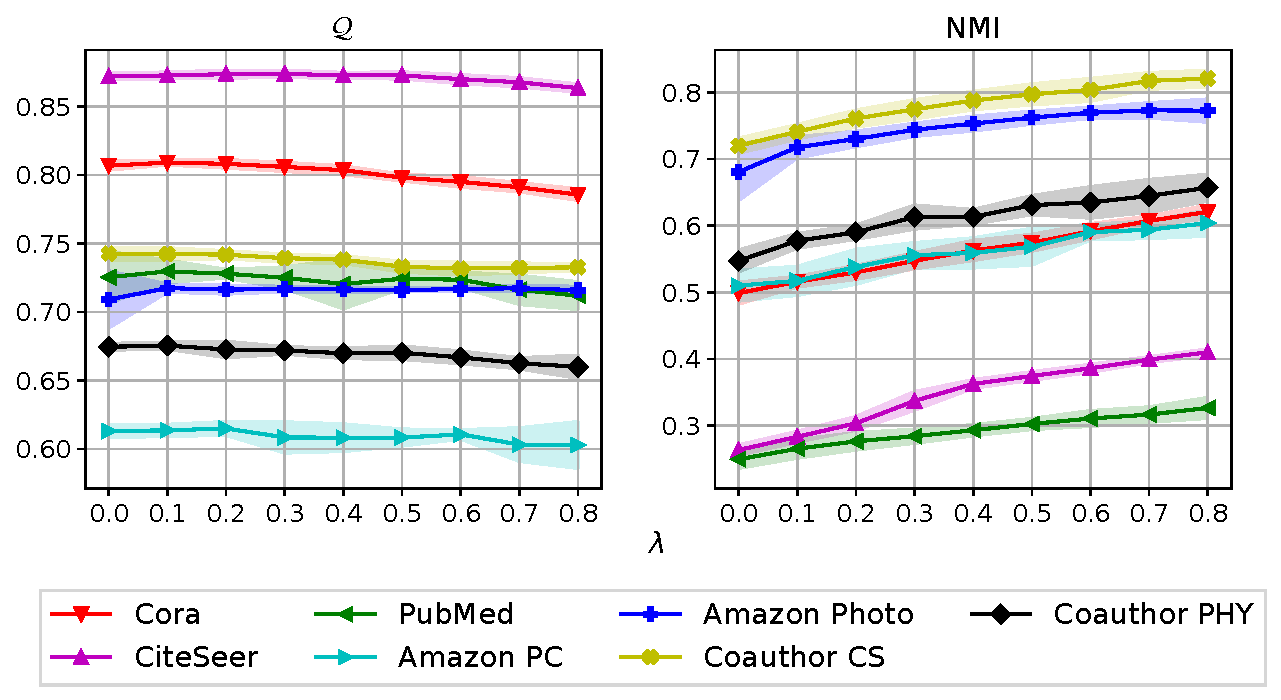
\includegraphics[width=0.45\textwidth]{figures/results_modularity_nmi.pdf}
    \caption{Effect of auxiliary information on different metrics and datasets with varying $\lambda$. As expected, $Q$ tends to decrease as $\lambda$ increases since $Q$ is dependent only on the graph structure whereas $\lambda$ adds weight to the label-based loss. The NMI increases as $\lambda$ increases since NMI is directly related to labels.}
    \label{fig:lambda_effect_on_modularity_nmi}
\end{figure}


\subsection{Auxiliary Information Effect}

To check the effect of our auxiliary information, we vary the $\lambda$ hyperparameter in our additional experiments. Figure \ref{fig:lambda_effect_on_modularity_nmi} illustrates the impact of the hyperparameter on different metrics and datasets. The main goal of the $\lambda$ parameter is to find the best underlying partition leveraging both graph structure and auxiliary information. We can see modularity $Q$ has a consistent value over increased $\lambda$, while NMI values are increasing with a good amount. This shows the power of our auxiliary objective which ensures flexibility to the user aiming to optimize their desired metric. Additionally, the standard deviation of our results is small showing the stability of our algorithm.

\begin{table}[htbp]
\centering
\resizebox{0.47\textwidth}{!}{
\begin{tabular}{ccccccc}
\toprule
 & \multicolumn{2}{c}{\textsc{Cora}} & \multicolumn{2}{c}{\textsc{Citeseer}} & \multicolumn{2}{c}{\textsc{Pubmed}} \\ \midrule
\model & $Q \uparrow$ & NMI $\uparrow$ & $Q \uparrow$ & NMI $\uparrow$ & $Q \uparrow$ & NMI $\uparrow$ \\
\midrule
$\alpha=0.0$ & 80.8 & 43.5 & 87.4 & 22.2 & 72.8 & 30.1 \\
$\alpha=0.5$ & 80.8 & 40.3 & 87.3 & 20.3 & 72.1 & 28.1 \\
$\alpha=1.0$ & 80.8 & 38.5 & 87.4 & 19.5 & 71.7 & 26.3 \\
\bottomrule
\end{tabular}
}
\caption{Performance of our method with varying $\alpha$ regularization parameter. Additional regularization has a negligible effect while avoiding potential trivial clustering.}
\label{tab:additional_regularization}
\end{table}

\subsubsection{Additional Regularization}
In addition to the primary and the auxiliary information objective terms, we propose another regularization term, the squared average node similarity, $ \alpha(\frac{1}{n^2}\sum_{ij} \langle X_iX_j \rangle)^2= \alpha\|\bar{X}\|_2^4$, where $\bar{X}$ is the mean of the node embedding vectors and $\alpha$ is a tunable parameter. This regularizer can be used to avoid the formation of a trivial clustering where all the nodes form a single cluster. Table \ref{tab:additional_regularization} shows that adding this regularizer have a negligible effect on our main objectives while avoiding potential trivial clustering.

\begin{figure}[ht]
    \centering
    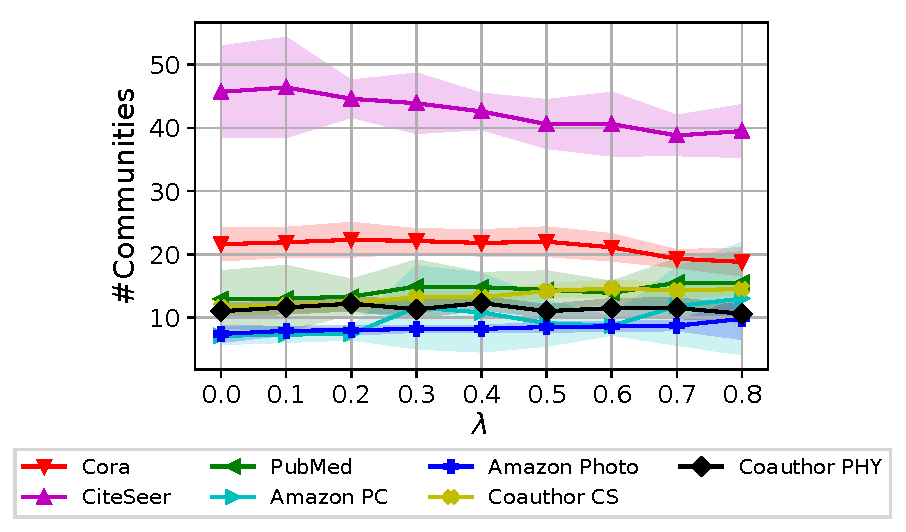
\includegraphics[width=0.42\textwidth]{figures/results_number_clusters.pdf}
    \caption{The number of communities varying $\lambda$ hyperparameter for different datasets. We observe that the number of communities found is similar across different $\lambda$ values except in some cases.}
    \label{fig:lambda_effect_on_number_of_communities}
\end{figure}

\subsection{Number of Communities}

Our method does not assume the number of communities in the data, which is one of its main strengths. The number of communities in real-world data is generally unknown, and it is nontrivial to estimate it. To share some insight, we provide the number of communities our method finds across different datasets and $\lambda$ values. Figure \ref{fig:lambda_effect_on_number_of_communities} demonstrates the number of communities varies for different datasets, and the results are consistent across different $\lambda$ values.















